\documentclass[pss]{wiley2sp} % provides pss two-column style
\usepackage{amsmath}
\usepackage{subfig}

\renewcommand{\arraystretch}{1.2} % please do not remove or change
\tolerance=400
\emergencystretch=10pt

\begin{document}


% Title of the article
\title{Nonlinear optical responses in hydrogenated graphene structures}

% Authors
\author{
Reinaldo Zapata-Pe\~na\textsuperscript{\Ast,\textsf{\bfseries 1}},
Sean M. Anderson\textsuperscript{\Ast,\textsf{\bfseries 1}},
Bernardo S. Mendoza\textsuperscript{\Ast,\textsf{\bfseries 1}},
Anatoli I. Shkrebtii\textsuperscript{\textsf{\bfseries 2}}}

% Abbreviated list of authors for the page headers
\titlerunning{Optical spin injection, current injection, and SHG study of
hydrogenated graphene}
\authorrunning{R. Zapata-Pe\~na et al.}

%E-mail-address of corresponding author
\mail{e-mail
  \textsf{bms@cio.mx}, Phone:
  +52-477-441-4200, Fax: +52-477-441-4209}

% author's affiliations/addresses
\institute{%
  \textsuperscript{1}\,Centro de Investigaciones en \'Optica, Le\'on,
  Guanajuato 37150, M\'exico\\
  \textsuperscript{2}\,University of Ontario, Institute of Technology, Oshawa,
  ON, L1H 7L7, Canada}

\received{XXXX, revised XXXX, accepted XXXX}
\published{XXXX} % do not change, will be filled in by the publisher

% Please select about four verbal keywords for your manuscript.
\keywords{graphene, spin polarization, current injection, second-harmonic.}

\abstract{%
\abstcol{%
We present a theoretical study of spin and current injection, and second-harmonic generation via optical means from the C$_{16}$H$_{8}$-alt and C$_{16}$H$_{8}$-up graphene structures. The incidence of circularly polarized light onto nonmagnetic semiconductors produces spin-polarized electrons in the conduction bands. Current injection and second-harmonic generation are nonlinear, second-order effects that can be produced from both the bulk and surface of noncentrosymmetric materials. In centrosymmetric materials, these effects can only be observed at the surface where the inversion symmetry is broken.} 
{We also report results for the degree of spin polarization, current injection, and second-harmonic generation calculated within a full electronic band structure scheme at the DFT-LDA level using a planewave basis. Our results show that these effects can be optically generated in both the C$_{16}$H$_{8}$-alt and C$_{16}$H$_{8}$-up structures, presenting an anisotropic behavior. We obtain a maximum degree of spin polarization of 39\% for C$_{16}$H$_{8}$-alt, and 57\% for C$_{16}$H$_{8}$-up, which are promising results for potential applications in spintronics.}
}


\maketitle


\section{Introduction}\label{sec:intro}

Graphene is an allotrope of carbon with a planar, hexagonal, two-dimensional
honeycomb structure with one carbon atom at each vertex (Fig.
\ref{fig:structures}) that has attracted great interest due to its distinctive
properties, such as the fractional quantum Hall effect at room temperature,
and excellent thermal transport properties
\cite{geimNM07,geimNM07,reinaNL08,bottegoniAPL13,balandinNL08}. It behaves
like a metal, but can be modified to semiconductor behavior by tuning the band
gap. This can be acheived by changing the surface area \cite{hanPRL07},
applying an electric field \cite{zhangN09}, applying uniaxial strain
\cite{niACSN08}, or by doping. amongst other methods. Previous works have
explored doping with boron, nitrogen \cite{guoIJ11}, and hydrogen
\cite{eliasS09,guisingerNL09,samarakoonACSN10}.

Hydrogenated graphene can obtain different spatial configurations by varying
the amount and location of the hydrogen bonds. In this paper we present a
study of two 50\% hydrogenated graphene structures, C$_{16}$H$_{8}$-alt and
C$_{16}$H$_{8}$-up (Figs. \ref{fig:altstrc} and \ref{fig:upstrc}), both
presenting a discernible band gap. When a hydrogen atom is bonded to a carbon
atom in graphene, it draws the atom away from the plane. This modifies the
carbon-carbon bond length and consequently expands the band gap
\cite{samarakoonACSN10}. The C$_{16}$H$_{8}$-alt case has hydrogen on both
sides of the carbon sheet, alternating between the upper and lower faces,
while the C$_{16}$H$_{8}$-up case has all the hydrogens on a single side,
producing a zig-zag form in the carbon lattice. We conduct a theoretical study
of three optical nonlinear phenomena for our two cases: the optical spin
injection, the optical current injection, and second-harmonic generation
(SHG). We describe these as follows.


\begin{figure}[t]
\subfloat[Top and side view of pristine graphene.]
{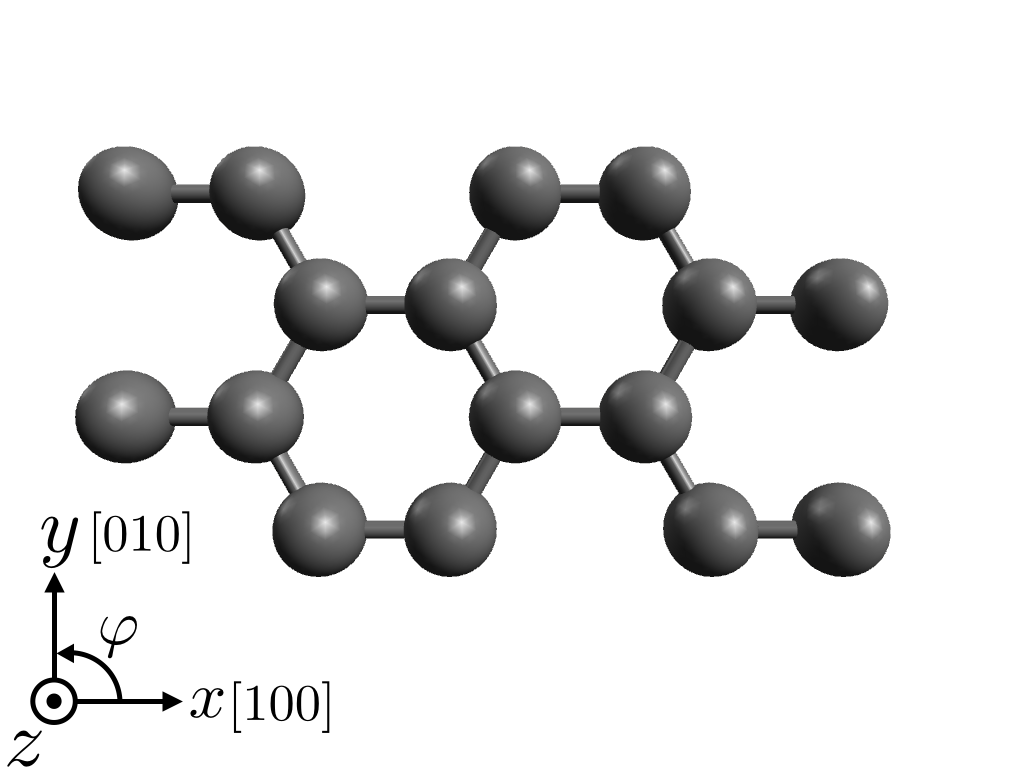
\includegraphics[width=0.49\linewidth]{figures/images/graph1}
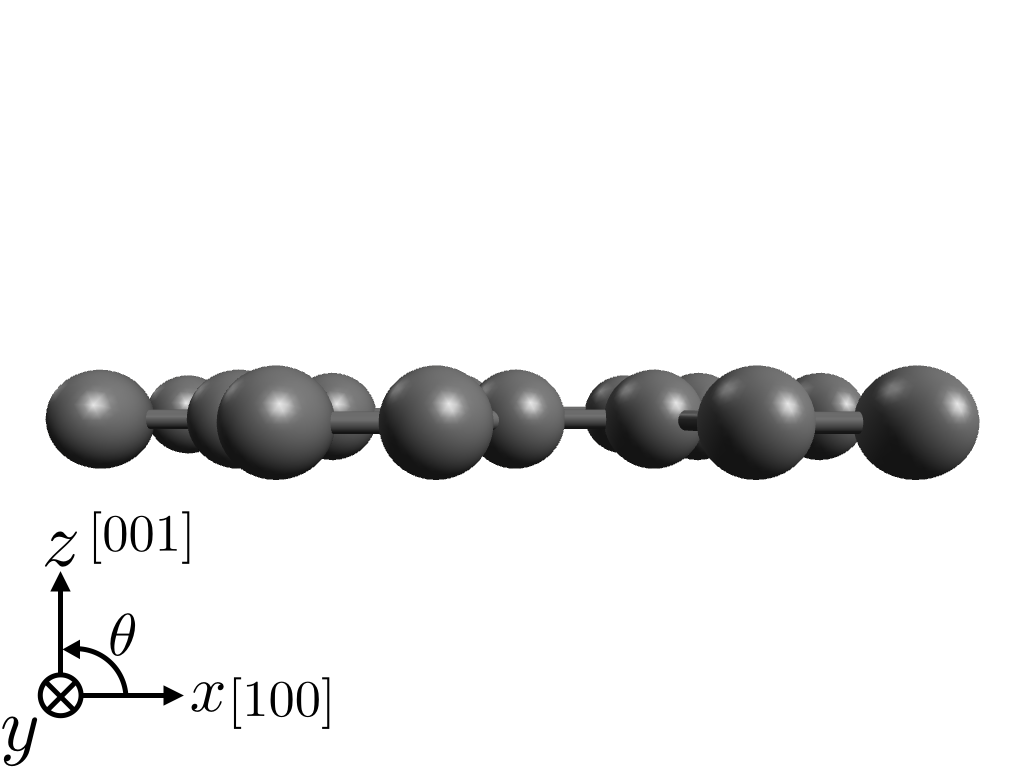
\includegraphics[width=0.49\linewidth]{figures/images/graph2}\label{fig:graphenestrc}}
\\
\subfloat[Top and side view of C$_{16}$H$_{8}$-alt graphene structure.]
{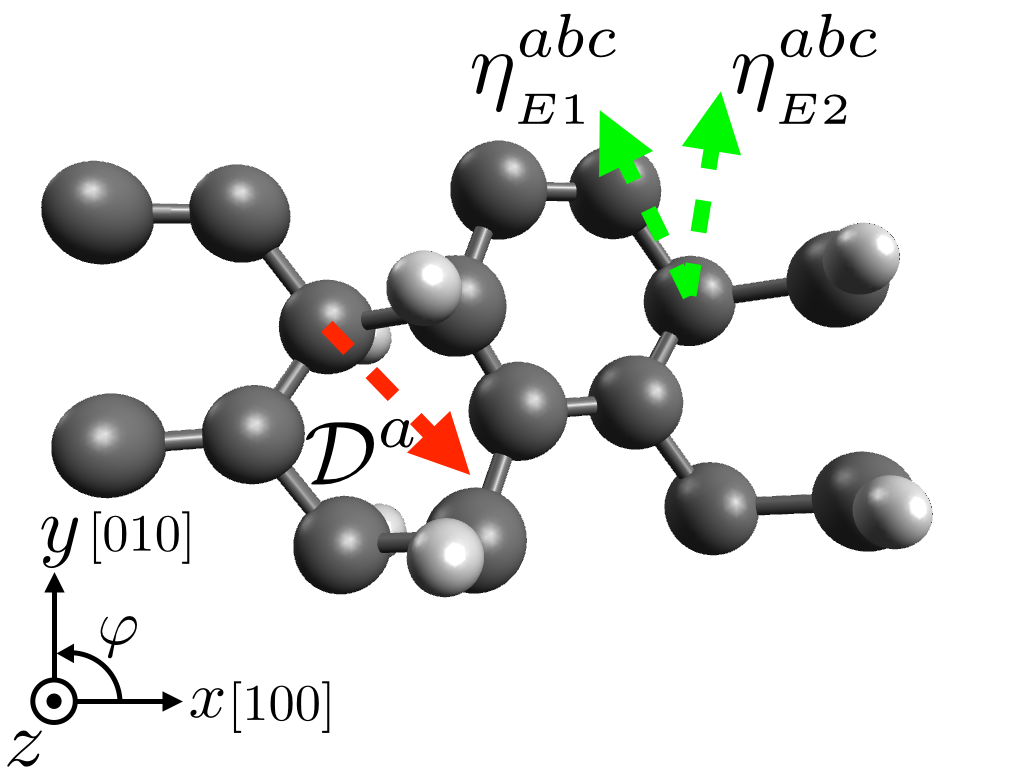
\includegraphics[width=0.49\linewidth]{figures/images/alt1}
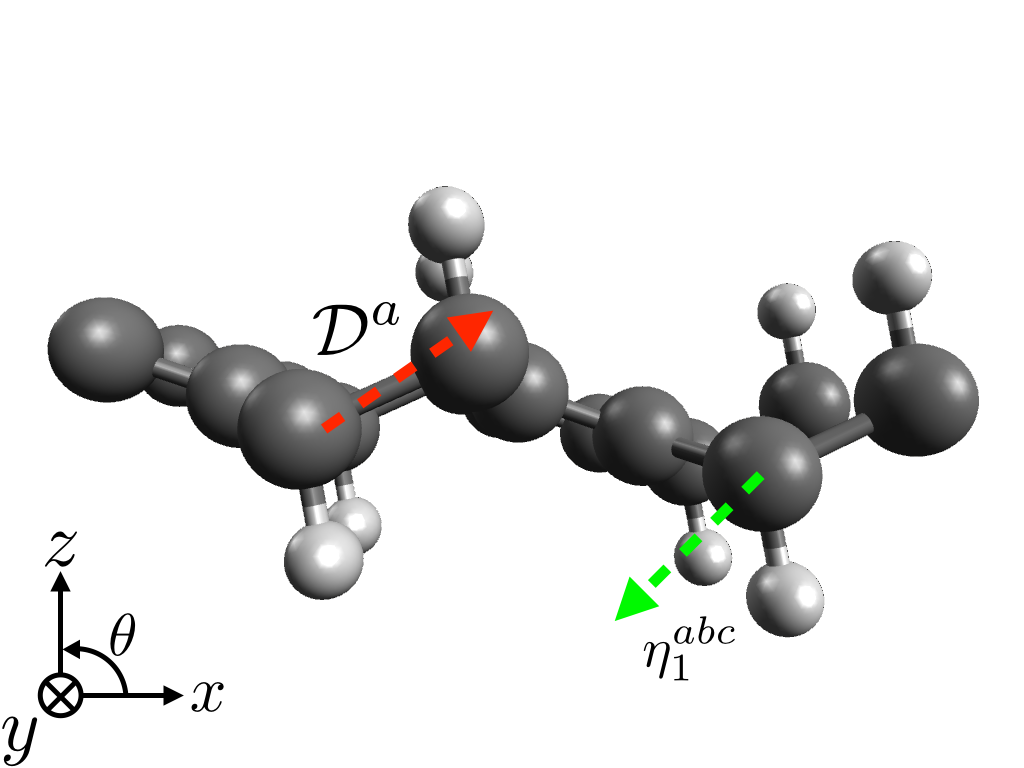
\includegraphics[width=0.49\linewidth]{figures/images/alt2}\label{fig:altstrc}}
\\
\subfloat[Top and side view of C$_{16}$H$_{8}$-up graphene structure.]
{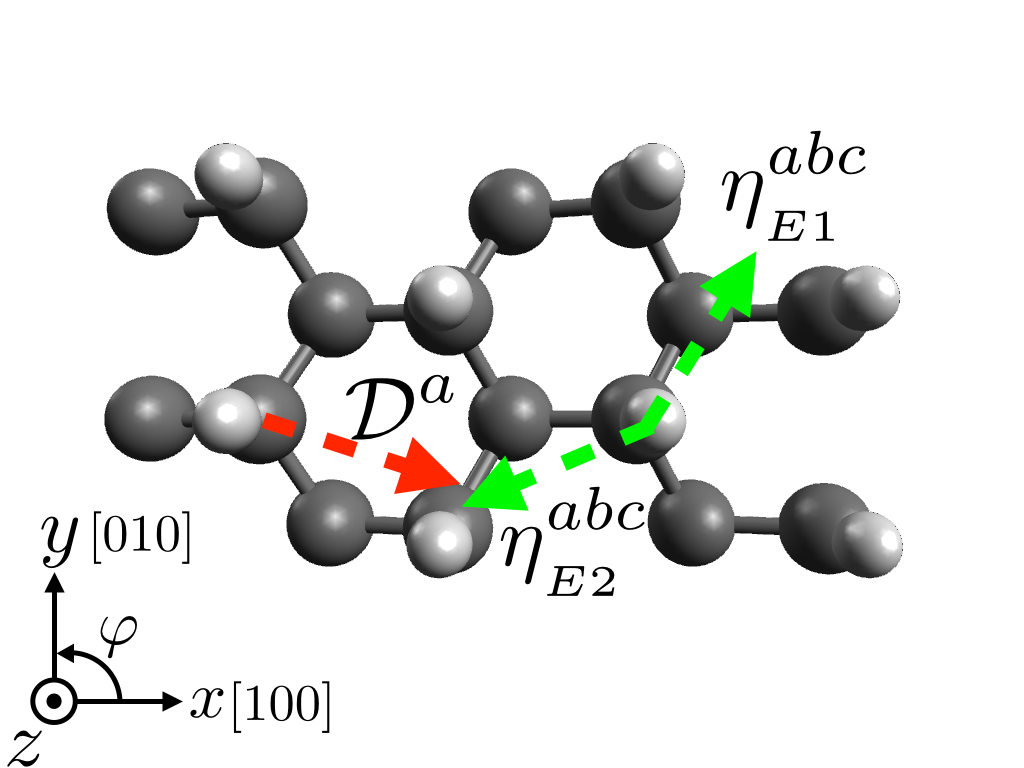
\includegraphics[width=0.49\linewidth]{figures/images/up1}
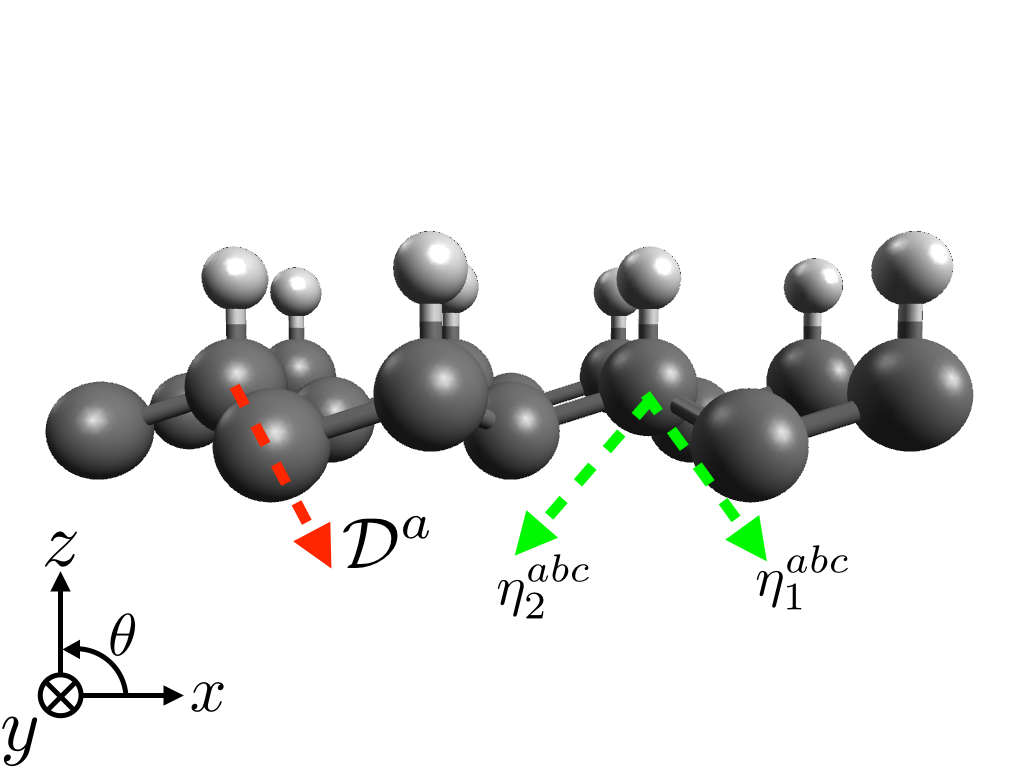
\includegraphics[width=0.49\linewidth]{figures/images/up2}\label{fig:upstrc}}
\caption{(Color online) Diagrams of pristine graphene
(\ref{fig:graphenestrc}), and the C$_{16}$H$_{8}$-alt (\ref{fig:altstrc}), and
C$_{16}$H$_{8}$-up (\ref{fig:upstrc}) structures. The light (dark) spheres
correspond to hydrogen (carbon) atoms. We take the honeycomb lattice to be in
the $xy$ plane, and the carbon plane itself to be in the $xz$
plane.\label{fig:structures}}
\end{figure}

% The red (green) dashed arrows in \ref{fig:altstrc} and \ref{fig:upstrc}
% represent the direction where the $\mathcal{D}(\omega)$
% ($\eta^{abc}(\omega)$) point in the corresponding $xy$ and $xz$ plane. This
% information is explained in subsections \ref{subsec:results-DSP} and
% \ref{subsec:results-eta}.


\subsection{Optical spin injection}

The injection and detection of spin polarized electrons into nonmagnetic
materials is the core of spintronics \cite{vzuticRMP04,fertRMP08} and an
important  problem in condensed matter theory. Our concern is with the
production of spin polarization from light \cite{LampelPRL68}, and this
conversion from the angular momentum of light into electron spin is very
efficient in III-IV semiconductors \cite{dyakonovOO84}. The optical spin
injection is characterized through the degree of spin polarization (DSP)
$\mathcal{D}(\omega)$, which is a dimensionless quantity and a function of the
photon frequency $\omega$. The DSP quantifies the fraction of injected
electrons into the conduction bands that are spin polarized. This effect
occurs when circularly polarized light is incident on a semiconducting
material \cite{dyakonovOO84}, thus allowing electrons to move from the valence
to the conduction bands. The resulting polarization is produced by the
interaction between the electron spin and its motion caused by the spin-orbit
coupling in the material. DSP can be calculated with a full band structure
local-density approximation (LDA) and $\textbf{k}\cdot\textbf{p}$ methods
\cite{nastosPRB07,cabellosPRB09}. There are theoretical reports of DSP
calculations for bulk media (Si, GaAs, CdSe, and Ge semiconductors)
\cite{nastosPRB07,cabellosPRB09} and surfaces (Si(111):In, Si(111):As,
GaAs(110):Sb, GaAs(110), and Si(111) with $4\times2$ and $8\times2$
reconstructions) \cite{mendozaPRB12,arzatePRB14}.


\subsection{Optical current injection}

The optical current injection $\mathbf{\dot{J}}(\omega)$, is a surface-
sensitive optical effect that offers the potential to control chemical
reactions \cite{bhatPRB05,hachePRL97}. A photocurrent can be injected with a
single optical beam in noncentrosymmetric materials. This current results from
the interference of one-photon absorption processes associated with different
linear polarizations of the light. In the process of current injection, the
energy increase of the injected carriers is provided by the electromagnetic
field; meanwhile, the increase in momentum is provided by the crystal lattice
\cite{arzatePRB14}. From the total 32 crystal classes, 21 are
noncentrosymmetric, and 18 of these have a nonzero current injection. Crystal
classes $\bar{6}m\bar{2}$, $\bar{6}$, and $\bar{4}$$\bar{3}$m are the
exceptions \cite{sipePRB00}. The one-photon current injection is characterized
by the current injection tensor, $\eta(0;\omega,−\omega)$, which is a
particular case of $\eta(\omega_{1}-\omega_{2};\omega_{1},-\omega_{2})$, where
$\omega_{1}$ and $\omega_{2}$ are the frequencies of two different optical
fields. Henceforth, we will denote this tensor as $\eta(\omega)$ for ease of
notation. This phenomenon has been studied in bulk semiconductors
\cite{hachePRL97,sipePRB00}, two-dimensional systems
\cite{melePRB00,cabellosPRB11}, and one-dimensional nanotubes
\cite{melePRB00}.


\subsection{Second-harmonic generation}

The characterization of embedded structures and interfaces is an important
issue in the development of microelectronics, nanomaterials, semiconductors,
and other areas of interest in science and technology. Second-harmonic
generation (SHG) is a nonlinear process in which two photons of frequency
$\omega$ are destroyed, and a photon of frequency $2\omega$ is simultaneously
created. In the dipole approximation SHG is restricted to the surfaces of
centrosymmetric materials, making it an excellent surface probe. SHG
spectroscopy techniques bring the possibility to study properties of materials
and has a non invasive, nondestructive and surface sensitive nature. It is
possible to characterize properties like phase transitions, atomic structure,
molecular and atomic physisorption, structure deformation, and many others
\cite{dadapPRB97,godefroyAPL96,salazarPRB14,mendozaPRL98}. Theses techniques
work in non-ultrahigh vacuum conditions and can access interfaces that are
buried under transparent overlayers. The two cases in this study,
C$_{16}$H$_{8}$-alt and C$_{16}$H$_{8}$-up, are noncentrosymmetric and thus
present SHG from the entire structure.

This paper is organized as follows. In Sec. \ref{sec:theory} we present the
theory and formulas that describe the DSP, optical current injection, and SHG.
In Sec. \ref{sec:results} we describe the details of the calculations and the
corresponding spectra for the respective \emph{alt} and \emph{up} structures.
Finally, we give our conclusions in Sec. \ref{sec:conclusions}.


\section{Theory}\label{sec:theory}

In this section we report a summary of the theory for the three phenomena of
interest. For full details see Refs. \cite{nastosPRB07,mendozaPRB12} for DSP,
Refs. \cite{cabellosPRB11,sipePRB00} for optical current injection, and Ref.
\cite{andersonPRB15} for SHG.


\subsection{Optical spin injection}\label{sec:theory-DSP}

The optical spin injection is characterized by the DSP, $\mathcal{D}(\omega)$.
Along a given direction $a$, we write the DSP \cite{cabellosPRB09} as
\begin{equation}\label{eq:da}
\mathcal{D}^{a}(\omega)=
\frac{\dot{S}^{abc}(\omega)}{(\hbar/2)\dot{n}^{bc}(\omega)},
\end{equation}
where the superscripts denote the three Cartesian directions. The spin
generation rate, $\dot{S}^{abc}(\omega)$, and the carrier generation rate,
$\dot{n}^{bc}(\omega)$, are given by
\begin{align*}
\dot{S}^{abc}(\omega)&= 
\zeta^{abc}(\omega)E^{b}(-\omega)E^{c}(\omega),\nonumber\\
\dot{n}^{bc}(\omega)&= 
\xi^{bc}E^{b}(-\omega)E^{c}(\omega),
\end{align*}
where $\zeta^{abc}(\omega)$ is the spin injection rate tensor and
$\xi^{bc}(\omega)$ is the carrier generation rate tensor. The spin injection
rate tensor is given by
\begin{align*}\label{eq:zeta}
\zeta^{abc}(\omega) &= \frac{i\pi e^{2}}{\hbar^{2}}\int\frac{d^{3}k}{8\pi^{3}}
\sum_{vcc'}^{\prime}\text{Im}\bigl[S^{a}_{c'c}(\textbf{k})
r^{b}_{vc'}(\textbf{k})r^{c}_{cv}(\textbf{k})\nonumber\\
&\qquad+S^{a}_{cc'}(\textbf{k})
r^{b}_{vc}(\textbf{k})r^{c}_{c'v}(\textbf{k})\bigr]
\delta(\omega_{cv}(\textbf{k})-\omega),
\end{align*}
where $S^{a}_{nm}$ and $r^{a}_{nm}$ are the spin and position matrix elements.
Lastly, the carrier generation rate tensor is related to the linear optical
response tensor by
\begin{equation*}
\xi^{bc}(\omega)=\mathrm{Im}[(2/\hbar)\chi^{bc}].
\end{equation*}
We assume an incoming circularly polarized beam at normal incidence that
propogates along the $-z$ direction, $\mathbf{E}(\omega) =
E_{0}(\omega)(\hat{x} - i\hat{y})/\sqrt{2}$. Then the expression of Eq.
\eqref{eq:da} can be reduced to \cite{arzatePRB14}
\begin{equation}\label{eq:D^i}
\mathcal{D}^{a}(\omega) = 
\frac{-4i\zeta^{axy}(\omega)}
    {\hbar\left[\xi^{xx}(\omega) + \xi^{yy}(\omega)\right]}.
\end{equation}
It is possible to generate current injection along all three orthogonal
directions with an incident circularly polarized beam and so the total DSP can
be obtained by \cite{arzatePRB14}
\begin{equation}\label{eq:dsptotal}
\mathcal{D}(\omega) =
\sqrt{[\mathcal{D}^{x}(\omega)]^{2} + 
      [\mathcal{D}^{y}(\omega)]^{2} +
      [\mathcal{D}^{z}(\omega)]^{2}
      }.
\end{equation}


\subsection{Optical current injection}\label{sec:theory-OCI}

The optical current injection is defined as
\begin{equation*}
\mathbf{\dot{J}}^{a}_{\text{inj}}(\omega) =
\eta^{abc}(\omega)E_{b}(\omega)E_{c}(\omega), \label{eq:eta}
\end{equation*}
where $\eta^{abc}(\omega)$ is the surface current injection tensor and is given by
\begin{align*}
\eta^{abc}(\omega) =& \frac{i\pi e^{3}}{\hbar^{2}}\int\frac{d^{3}k}{8\pi^{3}}
\nonumber \\
\times &
\sum_{vc}\mathrm{\Delta}^{a}_{cv}(\mathbf{k})\text{Im}\big[r^{b}_{cv}(\mathbf{k})
r^{c}_{cv}(\mathbf{k})\big]\delta(\omega_{cv}(\mathbf{k})-\omega).
\end{align*}
$r^{a}_{nm}$ is the position matrix elements and 
\begin{equation*}
\mathrm{\Delta}^{a}_{cv} = v^{a}_{cc}(\mathbf{k})-v^{a}_{vv}(\mathbf{k}),
\end{equation*}
where $v^{a}_{nn}(\mathbf{k})=p^{a}_{nn}(\mathbf{k})/m_{e}$ is the electron
velocity for a given $n$ band and the superscripts denote Cartesian
directions.

$\eta^{abc}(\omega)$ is purely imaginary and is antisymmetric with respect to
the last two indices \cite{sipePRB00,nastosPRB06}. Like in optical spin
injection, it is possible to generate current injection along all three
directions with an incident circularly polarized beam. Therefore, the only
components to be calculated are $\eta^{xxy}(\omega)$, $\eta^{yxy}(\omega)$,
and $\eta^{zxy}(\omega)$. Analogously to Eq.
\eqref{eq:dsptotal} it is possible to have the total $\eta(\omega)$ as
\begin{equation}\label{eq:etatotal}
\eta(\omega) =
\sqrt{[\eta^{xxy}(\omega)]^{2} +
      [\eta^{yxy}(\omega)]^{2} +
      [\eta^{zxy}(\omega)]^{2}
      }.
\end{equation}


\subsection{Second-harmonic generation}\label{sec:theory-SHG}

The formalism presented here for second order susceptibility tensor including
in one formulation (i) the scissors correction, (ii) the contribution of the
nonlocal part of the pseudopotentials, and (iii) the cut function for
selecting individual layer contributions \cite{andersonPRB15}. The second
order nonlinear polarization is given by
\begin{equation*}\label{eq:pol}
\mathcal{P}(2\omega) = 
\chi^{abc}(-2\omega;\omega,\omega)E^{b}(\omega)E^{c}(\omega)
\end{equation*}
where $\chi^{abc}(-2\omega;\omega,\omega)$ is the nonlinear susceptibility
tensor responsible for the SHG and satisfies permutation symmetry condition.
Again, the superscripts in the previous expression denote the Cartesian
directions and if repeated are to be summed over. The expressions for the
imaginary part of the tensor components $\chi^{abc}(-2\omega;\omega,\omega)$
for $1\omega$ and $2\omega$ are divided into interband ($e$) and intraband
($i$) as follows,
\begin{subequations}\label{eq:chis}
\begin{align}
\mathrm{Im}[\chi^{abc}_{e,\omega}] =  
\frac{\pi |e|^3}{2\hbar^2}\int 
&
\frac{dk^3}{8\pi^3}  
\nonumber \\
\times \sum_{vc}\sum_{q\neq(v,c)}
\frac{1}{\omega^\mathrm{\Sigma}_{cv}}
&
\left[\frac{\mathrm{Im}[\mathcal{V}^{\mathrm{\Sigma},a}_{qc}\{r^{b}_ 
{cv}r^{c}_{vq}\}]}
{(2\omega^\mathrm{\Sigma}_{cv}-\omega^\mathrm{\Sigma}_{cq})}\right.
\nonumber \\
& 
\left. -\frac{\mathrm{Im}[\mathcal{V}^{\mathrm{\Sigma},a}_{vq}\{r^{c}
_{qc}r^{b}_{cv}\}]}
{(2\omega^\mathrm{\Sigma}_{cv}-\omega^\mathrm{\Sigma}_{qv})}
\right]\delta(\omega^\mathrm{\Sigma}_{cv}-\omega),
\end{align}

\begin{align}
\mathrm{Im}  [\chi^{abc}_{i,\omega}]= 
\frac{\pi\vert e\vert^3}{2\hbar^2}
&
\int \frac{dk^3}{8\pi^3} 
\nonumber \\
 \times \sum_{cv}\frac{1}{(\omega^\mathrm{\Sigma}_{cv})^{2}} 
&
\Bigg[
\mathrm{Re}\left[\left\{r^{b}_{cv}\left(\mathcal{V}^
{\mathrm{\Sigma},a}_{vc}\right)_{;k^{c}}\right\}\right]
\nonumber \\
&+\frac{\mathrm{Re}\left[\mathcal{V}^{\mathrm{\Sigma},a}_{vc}\left\{
r^{b}_{cv}
\mathrm{\Delta}^{c}_{cv}\right\}\right]}{\omega^\mathrm{\Sigma}_{cv}} 
\Bigg]
\delta(\omega^\mathrm{\Sigma}_{cv}-\omega),
\end{align}

\begin{align}
\mathrm{Im}[\chi^{abc}_{e,2\omega}]= -
&
\frac{\pi |e|^3}{2\hbar^2}\int \frac{dk^3}{8\pi^3}
\nonumber \\
\times \sum_{vc}\frac{4}{\omega^\mathrm{\Sigma}_{cv}}
&
\Bigg[
\sum_{v'\ne v}\frac{\mathrm{Im}[\mathcal{V}^{\mathrm{\Sigma},a}_{vc}\{r^{b}
_{cv'}r^{c}_{v'v}\}]}
{2\omega^\mathrm{\Sigma}_{cv'}-\omega^\mathrm{\Sigma}_{cv}}
\nonumber \\ 
&
- \sum_{c'\ne c}
\frac{\mathrm{Im}[\mathcal{V}^{\mathrm{\Sigma},a}_{vc}
\{r^{c}_{cc'}r^{b}_{c'v}\}]}
{2\omega^\mathrm{\Sigma}_{c'v}-\omega^\mathrm{\Sigma}_{cv}}
\Bigg]
\delta(\omega^\mathrm{\Sigma}_{cv}-2\omega),
\end{align}

\begin{align}
\mathrm{Im}[\chi^{abc}_{i,2\omega}]= 
\frac{\pi \vert e\vert^{3}}{2\hbar^2}
&
\int \frac{dk^3}{8\pi^3}
\nonumber \\
\times \sum_{vc}\frac{4}{(\omega^\mathrm{\Sigma}_{cv})^{2}}
\Bigg[ 
&
\mathrm{Re}\left[\mathcal{V}^{\mathrm{\Sigma},a}_{vc}\left\{
\left(r^{b}_{cv}\right)_{;k^{c}}\right\}\right] 
\nonumber \\
-
&
\frac{2\mathrm{Re}
\left[\mathcal{V}^{\mathrm{\Sigma},a}_{vc}\left\{
r^{b}_{cv}
\mathrm{\Delta}^{c}_{cv}\right\}\right]}{\omega^\mathrm{\Sigma}_{cv}}
\Bigg]
\delta(\omega^\mathrm{\Sigma}_{cv}-2\omega)
,
\end{align}
\end{subequations}
where $\mathcal{V}^{\mathrm{\Sigma}}_{nm}$ is the velocity matrix elements,
that are derived from the complete velocity operator defined as
\begin{equation*}\label{eq:nonlocal}
\boldsymbol{\mathcal{V}}^{\mathrm{\Sigma}}\equiv
\boldsymbol{\mathcal{V}}+
\boldsymbol{\mathcal{V}}^{\mathrm{nl}}+
\boldsymbol{\mathcal{V}}^{S}.
\end{equation*}
$\boldsymbol{\mathcal{V}}^{\mathrm{nl}}$ includes the contribution from the
nonlocal part of the pseudopotentials, and $\boldsymbol{\mathcal{V}}^{S}$
includes the scissors correction. Lastly, $r^{a}_{nm}$ is the position matrix
elements, and $\omega^\mathrm{\Sigma}_{nm}$ =
$\omega^{\mathrm{\Sigma}}_{n}$-$\omega^{\mathrm{\Sigma}}_{m}$. The real part
of each contribution can be obtained through a Kramers-Kronig transformation
\cite{tancognePRB14} and
\begin{equation}\label{eq:chitotal}
\chi^{abc} (-2\omega;\omega,\omega) =
\chi^{abc}_{e,\omega} + \chi^{abc}_{e,2\omega} +
\chi^{abc}_{i,\omega} + \chi^{abc}_{i,2\omega}.
\end{equation}


\section{Results}\label{sec:results}

We present the results for {$D^{a}(\omega)$}, {$\eta^{abc}(\omega)$}, and
$\chi^{abc}(-2\omega;\omega,\omega)$ for the C$_{16}$H$_{8}$-alt and
C$_{16}$H$_{8}$-up structures. Both cases are semi-infinite carbon systems
with 50\% of hydrogenation in two different arrangements. The \emph{alt}
system has alternating hydrogen atoms on the upper and bottom sides of the
carbon sheet, while the \emph{up} system has H only on the upper side. Both
structures are noncentrosymmetric and have a thickness of 2.94\,{\AA} and
2.76\,{\AA}, respectively. The corresponding coordinates in Angstroms (\AA)
for the \emph{alt} and \emph{up} unit cells of the structures are presented in
Tables \ref{tab:altstrc} and \ref{tab:upstrc}. We establish our carbon plane
as the $xy$ plane for both structures. The hydrogen atoms are located over and
under the $xy$ plane. The hydrogen atoms are located above or below the carbon
plane in the $z$ direction, so we define the $xz$ plane identical to the side
view of the structure. See Fig. \ref{fig:graphenestrc}. The azimuthal angle
$\varphi$ is defined in the $xy$ plane and the polar angle $\theta$ in the
$xz$ plane.

\begin{table}[t]
% \sidecaption
\begin{tabular}{cccc}
\hline
Atom type &  \multicolumn{3}{c}{Position [\AA] } \\
\cline{2-4}
& $x$ & $y$ & $z$ \\
\hline
\multicolumn{2}{l}{First layer}\\
H & 2.460673853 & 0.342436286 & 13.741105571 \\
\multicolumn{2}{l}{Second layer}\\
C & 2.460673854 & 0.030828762 & 12.665048452 \\
C & 3.691010863 & 3.496845641 & 12.426806318 \\
C & 3.691010864 & 2.185854780 & 12.110583807 \\
C & 2.460673853 & 1.389876044 & 11.872402140 \\
\multicolumn{2}{l}{Third layer}\\
H & 2.460673853 & 1.078176853 & 10.796355805 \\
\hline
\end{tabular}
\caption[]{%
Atom types and positions for the C$_{16}$H$_{8}$-alt structure unit cell in
Cartesian coordinates. The system was separated into three layers: (i) top
hydrogen atoms, (ii) central carbon atoms, and (iii) bottom hydrogen atoms.
\label{tab:altstrc}}
\end{table}
\begin{table}[t]
% \sidecaption
\begin{tabular}{cccc}
\hline
Atom type &  \multicolumn{3}{c}{Position [\AA]} \\
\cline{2-4}
& $x$ & $y$ & $z$ \\
\hline
\multicolumn{2}{l}{First layer}\\
H &  -0.0000004500 & 0.001295619 & 25.719423746 \\
H & \ 2.3250097760 & 4.025098686 & 25.719040070 \\
\multicolumn{2}{l}{Second layer}\\
C & \ 2.3249742340 & 4.029801762 & 23.408608492 \\
C &  -0.0000004500 & 0.004159945 & 23.407634295 \\
C &  -0.0000004500 & 2.681215349 & 22.969636067 \\
C & \ 2.3250023170 & 6.706652267 & 22.953013267 \\
\hline
\end{tabular}
\caption[]{%
Atom types and positions for the C$_{16}$H$_{8}$-up structure unit cell in
Cartesian coordinates. The system was separated in two layers: (i) top
hydrogen atoms and (ii) bottom carbon atoms.}
\label{tab:upstrc}
\end{table}

We used the ABINIT code \cite{gonzeCPC09} for the calculation of the self-
consistent ground state and the Kohn-Sham states using density functional
theory in the local density approximation (DFT-LDA) with a planewave basis. We
used Hartwigsen-Goedecker-Hutter (HGH) relativistic separable dual-space
Gaussian pseudopotentials \cite{hartwigsenPRB98}that include spin-orbit
interaction for calculating $D^{a}(\omega)$. For the calculations of
{$\eta^{abc}(\omega)$} and $\chi^{abc}(-2\omega;\omega,\omega)$ we used
Troullier-Martins pseudopotentials \cite{troullierPRB91} that are fully
separable nonlocal pseudopotentials in the Kleiman-Bylander form
\cite{kleinmanPRL82}. The contribution from the nonlocal part of Eq.
\eqref{eq:nonlocal} is carried out using the DP code \cite{olevanoDP}. We used
cutoff energies of 65\,Ha and 40\,Ha for the \emph{alt} and \emph{up} cases,
respectively. The energy eigenvalues and matrix elements were calculated using
14452 \textbf{k} points and 8452 \textbf{k} points for the \emph{alt} and
\emph{up} cases, in the irreducible Brillouin zone (IBZ).


\subsection{Optical spin injection}\label{subsec:results-DSP}

In Fig. \ref{fig:Da} we show the $D^{a}(\omega)$ spectra for the
C$_{16}$H$_{8}$-alt and C$_{16}$H$_{8}$-up systems resulting from the
evaluation of the Eq. \eqref{eq:D^i}. Values over (under) zero define a
positive (negative) direction of spin polarization along the \emph{a}
direction with respect the three Cartesian vectors shown in Fig.
\ref{fig:structures}. For both cases, the onset of the response is when the
energy of the incoming light is the same as the gap energy. For the \emph{alt}
system this occurs at 0.72\,eV and for the \emph{up} system at 0.08\,eV. Both
cases have at least one direction with more than 30\% DSP. The \emph{alt}
system presents nearly 40\% $\mathcal{D}^{a}(\omega)$ in the $x$ and $y$
directions. Also, this structure presents an energy range between 0.720\,eV
and 0.722\,eV where it is possible to hold the maximum value for
$D^{a}(\omega)$ in all three directions. After 0.72\,eV the DSP rapidly
vanishes. Using Eq. \eqref{eq:dsptotal} we have that the \emph{alt} system
presents a total $\mathcal{D}(\omega)$=61\% for a frequency of 0.72\,eV with
$\varphi=-46^{\circ}$ and $\theta=35^{\circ}$. In Fig. \ref{fig:altstrc} the
dashed red arrow depicts how $\mathcal{D}(\omega)$ is oriented in the $xy$ and
$xz$ planes at the angles mentioned above.

For the \emph{up} structure we have nearly 60\% DSP in the $z$ direction. This
case also presents a range between 0.08\,eV to 0.084\,eV where it is possible
to hold the maximum values for $\mathcal{D}^{a}(\omega)$ for each component.
Using Eq. \eqref{eq:dsptotal} we have that the \emph{up} structure presents a
total $\mathcal{D}(\omega)$=64\% for a frequency of 0.08\,eV, with
$\varphi=-18^{\circ}$ and $\theta=-62^{\circ}$. In Fig. \ref{fig:upstrc} the
dashed red arrow depicts how $\mathcal{D}(\omega)$ is oriented in the $xy$ and
$xz$ planes at the angles mentioned above.

In Table \ref{tab:dacomp} we present a comparison of the absolute maximum
values of $\mathcal{D}^{a}(\omega)$ in a given direction for different
materials and the corresponding direction and energy at which they are
reached. From this table we have that the \emph{alt} and \emph{up} systems
have less DSP than the Si(111)-As 1$\times$1 and the the bulk CdSe cases, but
are comparable to the Si(111)-In 8$\times$2, bulk Si, and bulk GaAs systems.
Si(111)-In 8$\times$2 and \emph{alt} both have maxima around 0.72\,eV, which
is in the near infrared range. Conversely, the maxima for Si(111)-As
1$\times$1, bulk Si, and bulk GaAs all occur in the optical energy range. As
mentioned previously, the \emph{alt} and \emph{up} cases both have much larger
energy ranges for the maximum DSP values in all directions in comparison with
other structures. This compares very favorably with the other systems, that
have very narrow ranges over which the maximum DSP is achieved. The 0.7\,eV
maxima for \emph{alt} makes it an interesting candidate for further study, as
this energy is readily obtainable using terahertz radiation.

\begin{table}[b]
\sidecaption
\begin{tabular}{lcccc}
\hline
Case & Energy &  \multicolumn{2}{c}{$D^{a}$} &  Ref.\\
\cline{3-4}   & [eV]   & direction & [\%] \\
\hline
C$_{16}$H$_{8}$-alt  & 0.72 & y & 39  & * \\
C$_{16}$H$_{8}$-up   & 0.08 & z & 57  & * \\
Si(111)-In $8\times2$& 0.74 & z & 32  & \cite{arzatePRB14}\\
Si(111)-As $1\times1$& 2.20 & z & 100 & \cite{mendozaPRB12}\\
Bulk Si              & 3.44 & z & 30  & \cite{nastosPRB07}\\
Bulk GaAs            & 1.50 & z & 50  & \cite{nastosPRB07,bhatPRB05}\\
Bulk CdSe            & 1.80 & z & 100 & \cite{nastosPRB07}\\
\hline
\end{tabular}
\caption[]{Comparison of the reported absolute maximum values of {$D^{a}$} for
different materials. ($^{*}$This work)}
\label{tab:dacomp}
\end{table}

\begin{figure}[t]
\subfloat{\includegraphics[width=\linewidth]{figures/dsp-alt}}
\hfill
\subfloat{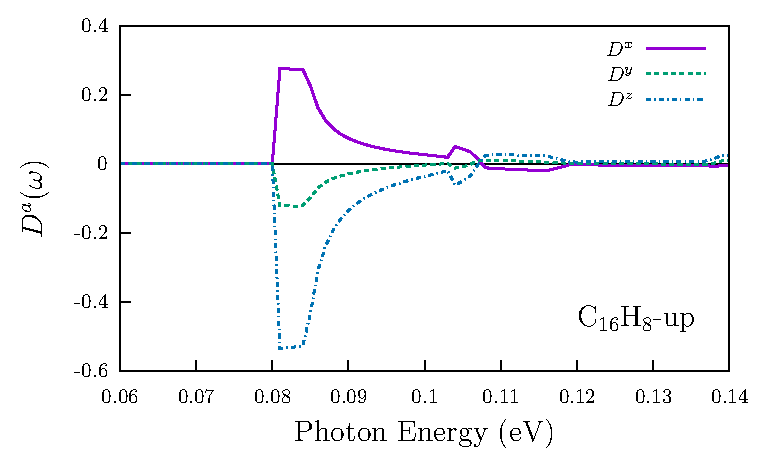
\includegraphics[width=\linewidth]{figures/dsp-up}}
\caption{(Color online) Spectra of the degree of spin polarization
{$D^{a}(\omega)$}, for the C$_{16}$H$_{8}$-alt and
C$_{16}$H$_{8}$-up.\label{fig:Da}}
\end{figure}


\subsection{Optical current injection}\label{subsec:results-eta}

Figs. \ref{fig:alt-eta} and \ref{fig:up-eta} depict the spectra obtained for
the current injection tensor components, $\eta^{xxy}(\omega)$,
$\eta^{yxy}(\omega)$, and $\eta^{zxy}(\omega)$ for the
\emph{alt} and \emph{up} systems. The \emph{alt} system is divided into three
layers comprised of the top H atoms, the carbon plane, and the bottom H atoms.
The \emph{up} system is divided into two layers comprised of the top H atoms
and the carbon plane. The layer selection for the unit cells are shown
explicitely in Tables \ref{tab:altstrc} and \ref{tab:upstrc}.

\begin{figure}[t]
\centering
\subfloat{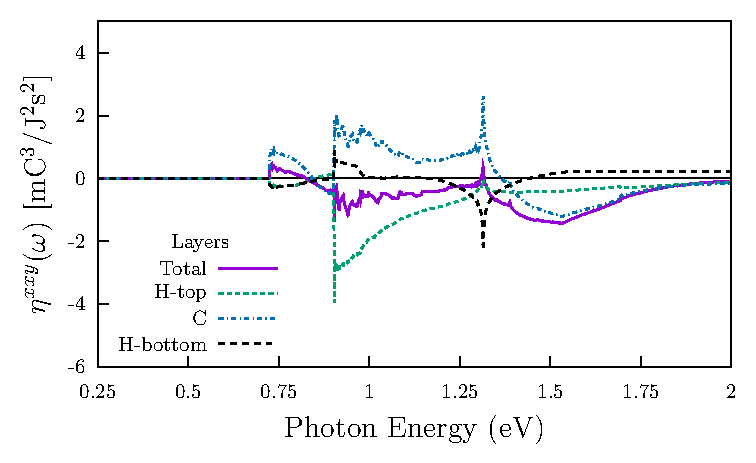
\includegraphics[width=\linewidth]{figures/eta-alt_x}}\\
\subfloat{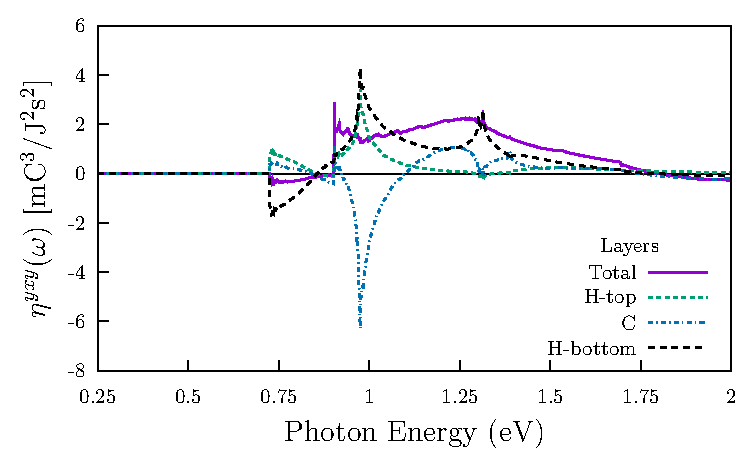
\includegraphics[width=\linewidth]{figures/eta-alt_y}}\\
\subfloat{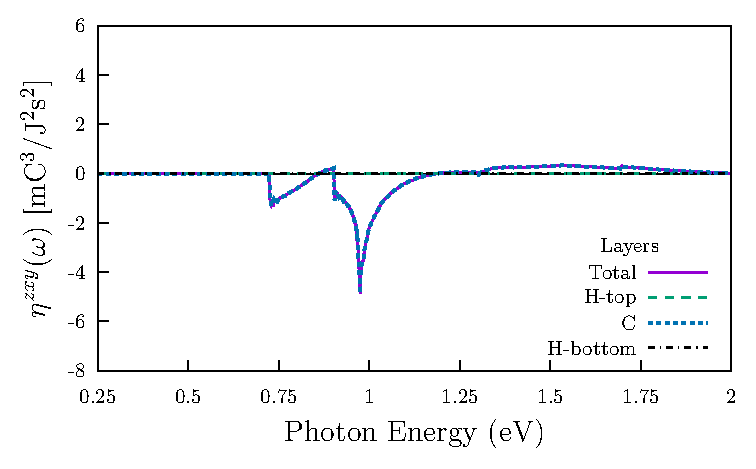
\includegraphics[width=\linewidth]{figures/eta-alt_z}}
% 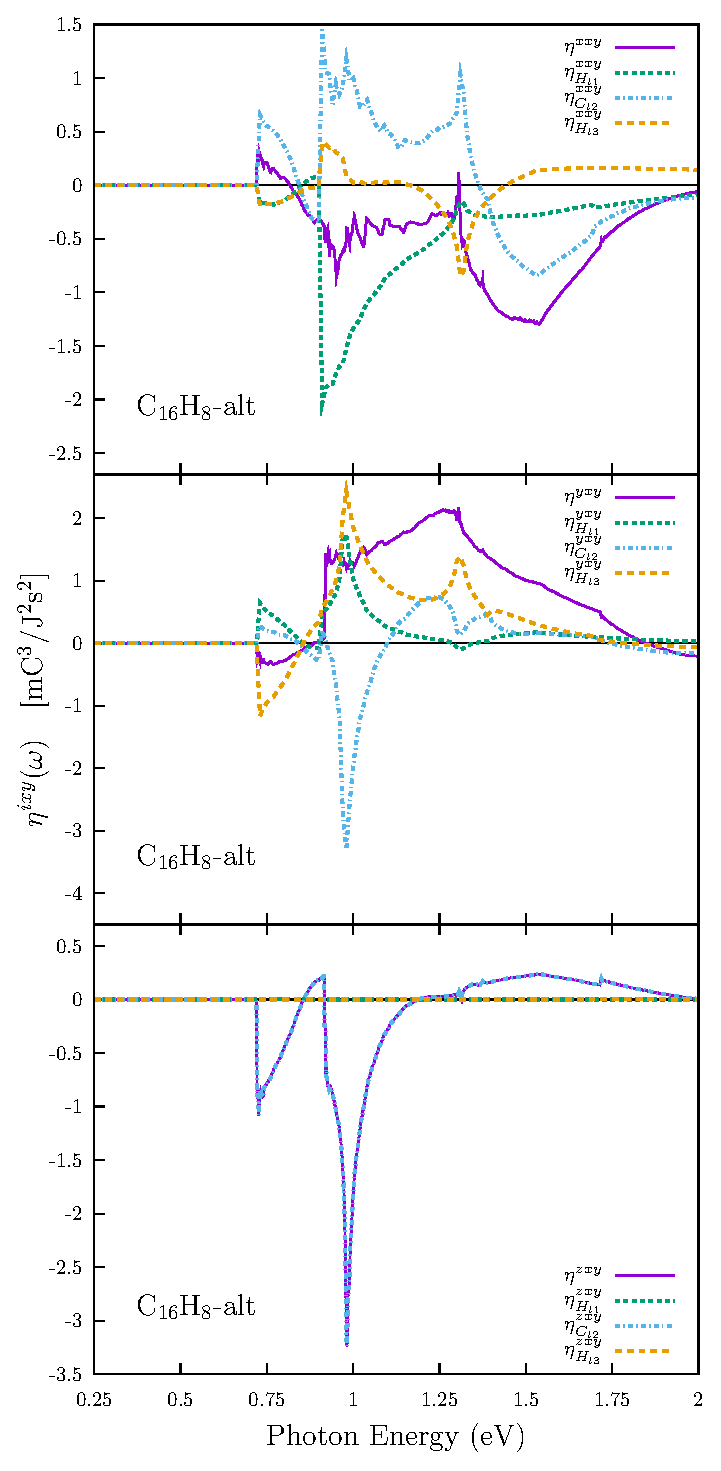
\includegraphics[width=\linewidth]{alt/alt-eta-layers}
\caption{(Color online) Spectra of the current injection tensor
{$\eta^{abc}(\omega)$} for C$_{16}$H$_{8}$-alt. Solid lines are the total
current injection and dashed lines correspond to the layer
contributions.\label{fig:alt-eta}}
\end{figure}

\begin{figure}[b]
\centering
\subfloat{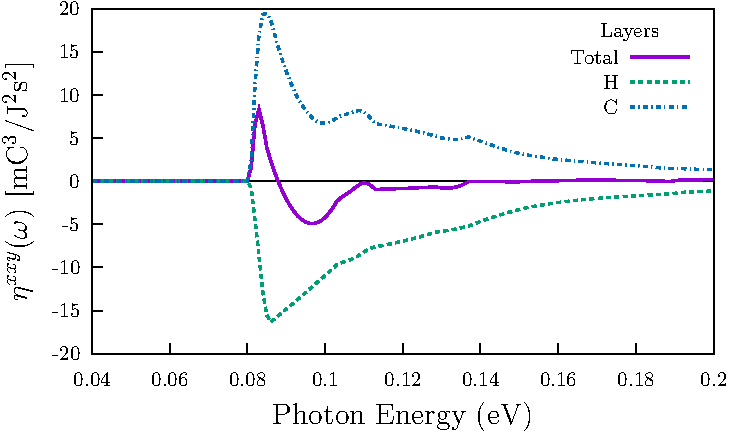
\includegraphics[width=\linewidth]{figures/eta-up_x}}\\
\subfloat{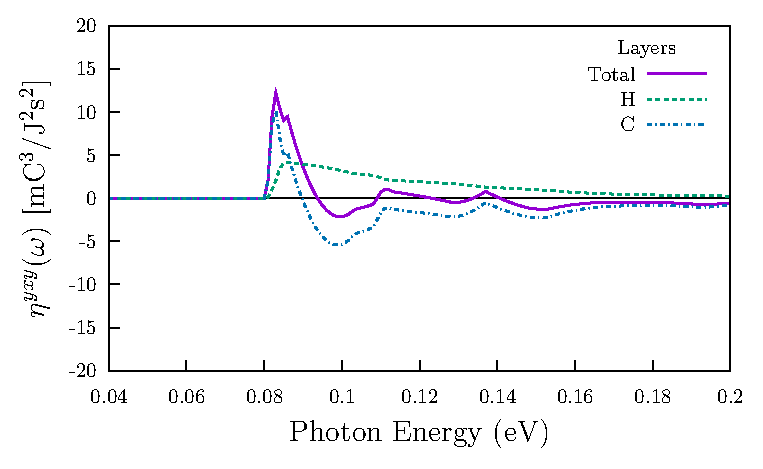
\includegraphics[width=\linewidth]{figures/eta-up_y}}\\
\subfloat{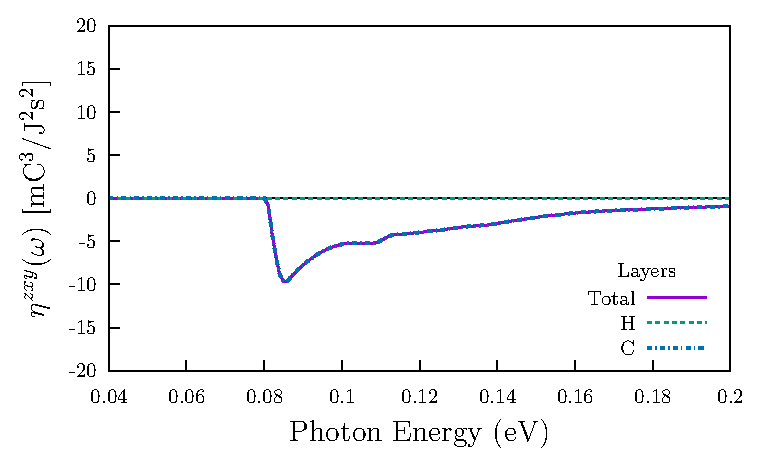
\includegraphics[width=\linewidth]{figures/eta-up_z}}
% 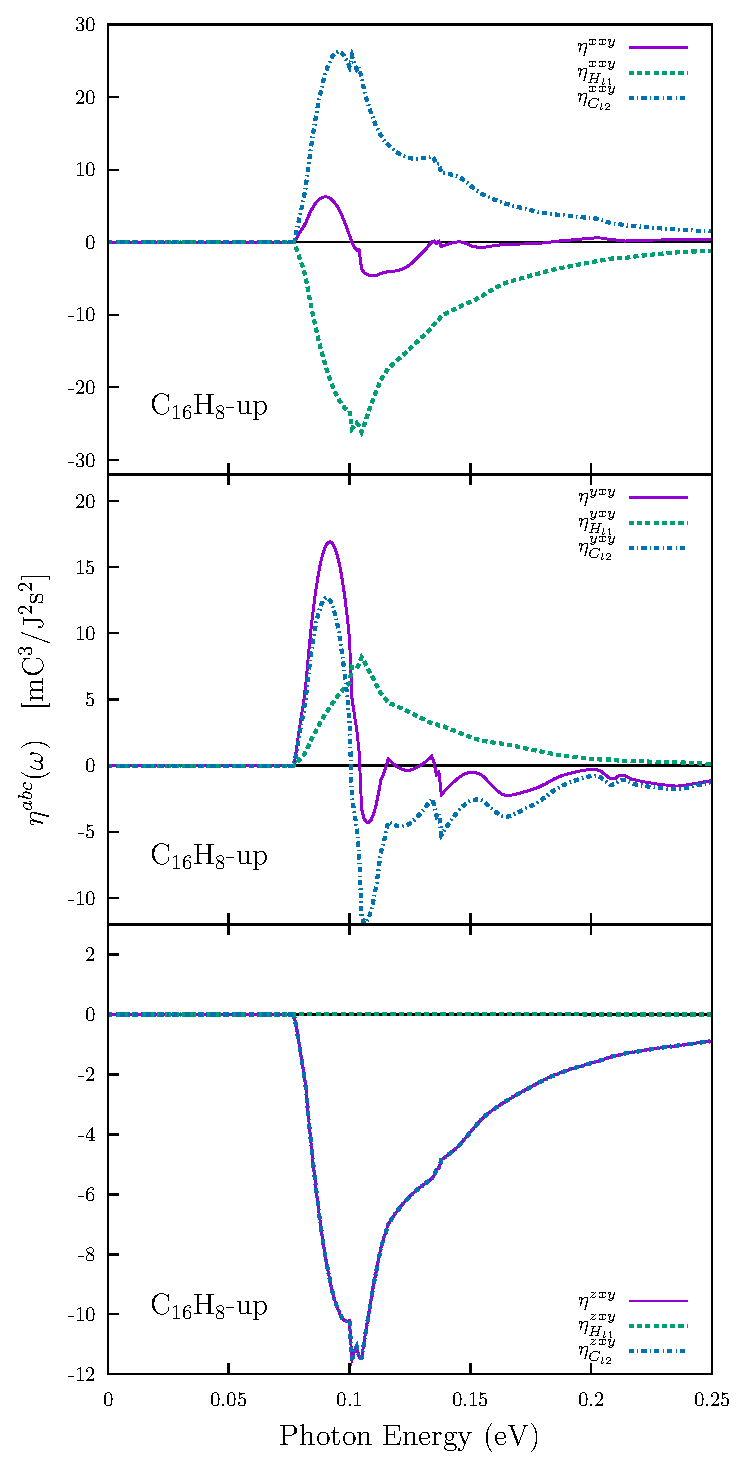
\includegraphics[width=\linewidth]{up/up-eta-multiplot}
\caption{(Color online) Spectra of the current injection tensor
{$\eta^{abc}(\omega)$} for C$_{16}$H$_{8}$-up. Solid lines are the total
current injection and dashed lines correspond to the layer
contributions.\label{fig:up-eta}}
\end{figure}

In Fig. \ref{fig:alt-eta} we present the three components for the full
\emph{alt} structure along with the layer by layer spectra. We establish two
energy values of interest for each structure where there are critical points
in the spectra. For the \emph{alt} structure we choose $E_{1} =
0.97\,\mathrm{eV}$ and $E_{2} = 1.31\,\mathrm{eV}$. For the layer by layer
analysis, we note that all three layers contribute toward $\eta^{xxy}(\omega)$
at $E_{1}$ with the carbon and top H layers providing the principal
contributions. For $E_{2}$, the dominating layers are the carbon and bottom H
layers with minimal contribution from the top H layer. For $E_{1}$, the
$\eta^{yxy}(\omega)$ component is also formed by contributions from all three
layers but dominated by the sum of the top and bottom H layers. The carbon
layer response is negative at that point, and destructively interferes with
the response from the other two layers. For $E_{2}$, the spectrum is
completely dominated by the bottom H layer, with almost no contribution from
the others. Lastly, at $E_{1}$ the $\eta^{zxy}(\omega)$ component is entirely
produced from the carbon layer, since the H layers provide no response
whatsoever. This component is negligible at $E_{2}$. We note that the response
for all three components vanishes after 1.75\,eV.

Using Eq. \eqref{eq:etatotal}, we find that the total current injection
$\eta(\omega)$, at $E_{1}$ is
$5.10\,\mathrm{mC}^{3}/\mathrm{J}^{2}\mathrm{s}^{2}$ with angles
$\varphi=116^{\circ}$ and $\theta=-172^{\circ}$. For $E_{2}$, we find that
$\eta(\omega)=2.32\,\mathrm{mC}^{3}/\mathrm{J}^{2}\mathrm{s}^{2}$ with angles
$\varphi=81^{\circ}$ and $\theta=12^{\circ}$. In Fig.
\ref{fig:altstrc}, the green dashed arrows represent the directions for
$\eta(\omega)$ for the $E_{1}$ and $E_{2}$ energy values. As mentioned
previously, $\varphi$ is located in the $xy$ plane, and $\theta$ is located in
the $xz$ plane.

Analogously, Fig. \ref{fig:up-eta} presents the three components for the full
\emph{up} structure along with the layer by layer spectra. We also establish
two energy values of interest for this structure, choosing $E_{1} =
0.09\,\mathrm{eV}$ and $E_{2} = 0.10\,\mathrm{eV}$. For $E_{1}$, the carbon
layer dominates the total response for all three components. For $E_{2}$, the
carbon layer dominates for both $\eta^{yxy}(\omega)$ and $\eta^{zxy}(\omega)$,
but both the H and carbon layer contribute significantly to
$\eta^{xxy}(\omega)$. Identically to the \emph{alt} structure, the
$\eta^{zxy}(\omega)$ component presents no response from the H layer.  We note
that the response for all three components vanishes after 0.2\,eV.

Using Eq. \eqref{eq:etatotal}, we find that the total current injection
$\eta(\omega)$, at $E_{1}$ is
$15.12\,\mathrm{mC}^{3}/\mathrm{J}^{2}\mathrm{s}^{2}$ with angles
$\varphi=58^{\circ}$ and $\theta=-54^{\circ}$. For $E_{2}$, we find that
$\eta(\omega)=7.62\,\mathrm{mC}^{3}/\mathrm{J}^{2}\mathrm{s}^{2}$ with angles
$\varphi=-157^{\circ}$ and $\theta=-131^{\circ}$. As before, present the
directions for $\eta(\omega)$ in Fig. \ref{fig:upstrc} using green dashed
arrows.

In Table \ref{tab:etacomp} we present a comparison of the maximum values of
different components of $\eta^{abc}(\omega)$ reported for different materials
and the corresponding energy at which they are achieved. Excluding bulk CdSe,
the \emph{alt} and \emph{up} structures have larger values for the current
injection tensor than the other materials. The Si(111)-In $8\times 2$ surface
has peak values close to 1.25\,eV, that is similar to the \emph{alt}
structure. However, the latter has more than six times the value of
$\eta^{yxy}(\omega)$.

In Ref. \cite{lamanAPL99} includes the results of a one-photon experiment for the optical current injection performed on bulk CdSe. They measured a current injection density of 2\,$\mu\mathrm{A}/\mathrm{cm}^{2}$ that entered 1.8\,$\mu\mathrm{m}$ deep. In Table \ref{tab:etacomp} we also show the corresponding experimental value for the surface current injection tensor of bulk CdSe.


\begin{table}%
\sidecaption
\begin{tabular}{lcccc}
\hline
Structure & Energy &  \multicolumn{2}{c}{$\eta^{abc}(\omega)$} &  Ref.\\
\cline{3-4}
          & [eV]   & $abc$ & [mC$^{3}$/J$^{2}$s$^{2}$] \\
\hline
C$_{16}$H$_{8}$-alt     & 1.28  & yxy & 2.25  & *     \\
C$_{16}$H$_{8}$-alt     & 0.97  & zxy & 4.86  & *     \\
C$_{16}$H$_{8}$-up      & 0.09  & yxy & 12.22 & *     \\
Si(111)-In $8\times2$   & 1.24  & yxy & 0.35  & \cite{arzatePRB14}  \\
Si(111) $2\times1$      & 0.75  & yxy & 1.22  & \cite{mendozaPRB12} \\
GaAs(110) clean         & 4.30  & yxy & 0.30  & \cite{nastosPRB07}     \\
GaS (110)-Sb            & 4.60  & yxy & 0.17  & \cite{cabellosPRB11}\\
Bulk CdSe               & 1.80  & yyz & 90.0$^{\star}$  & \cite{lamanAPL99}\\
\hline
\end{tabular}
\caption[]{%
Comparison of the highest reported absolute values of {$\eta^{abc}(\omega)$}
for different structures. ($^{*}$This work $^{\star}$Experimental value)}
\label{tab:etacomp}
\end{table}


\subsection{Second-harmonic generation}
In Figs. \ref{fig:alt-shg-abs} and \ref{fig:up-shg-abs} we show the absolute value of the different nonzero components of $\chi^{abc}$ for both cases resulting from the evaluation of Eqs. \eqref{eq:chis} and \eqref{eq:chitotal}. For the \emph{alt} system, we note that all components except $xxy$ present two peaks at $\sim0.5$\,eV and $\sim1.0$\,eV. The first peak is completely produced by $2\omega$ resonances, while the second peak is produced by a mixture of both $1\omega$ and $2\omega$ resonances, with the latter dominating in most cases. The $xxy$ component has a single broadened peak with a discernible feature near 0.5\,eV. That feature, much like the other components, is produced by $2\omega$ resonances, while the maxima is produced by a mixture of both frequencies, $1\omega$ and $2\omega$. For the \emph{up} structure we see one predominant peak around 0.05\,eV; it is completely produced by $2\omega$ transitions. The $xxy$ and $yxx$ components have an additional feature close to 0.09\,eV dominated by $1\omega$ transitions. In table \ref{tab:shgcomp} we show a comparison of the maximum $\chi^{abc}$ peak reported for different structures.
% 
% \begin{figure}[t]
% \subfloat{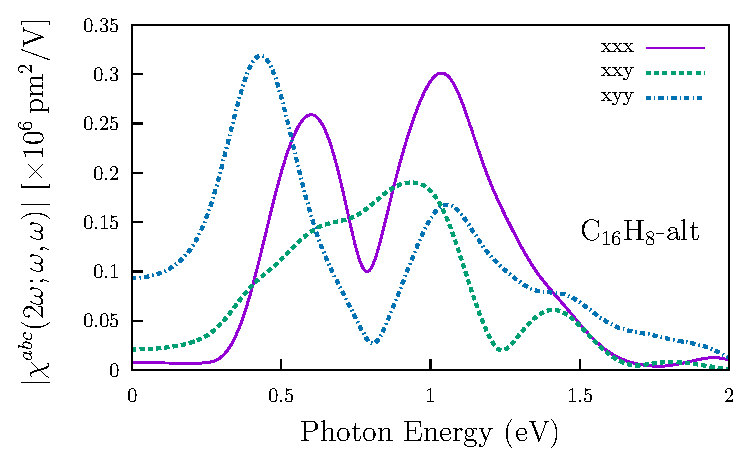
\includegraphics[width=\linewidth]{figures/alt_shg_abs_x}}\\
% \subfloat{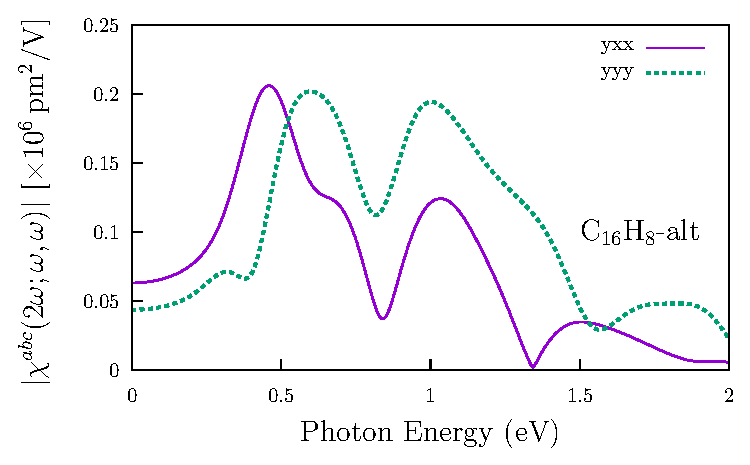
\includegraphics[width=\linewidth]{figures/alt_shg_abs_y}}
% \caption{(Color online) Spectra of the absolute value of SHG for the
    % C$_{16}$H$_{8}$-alt structure corresponding to the
    % sum of the absolute value for the non zero real and imaginary components
    % of $\chi^{abc}(2\omega;\omega,
    % \omega) $ tensor.\label{fig:alt-shg-abs}}
% \end{figure}
% 
% \begin{figure}[t]
% \subfloat{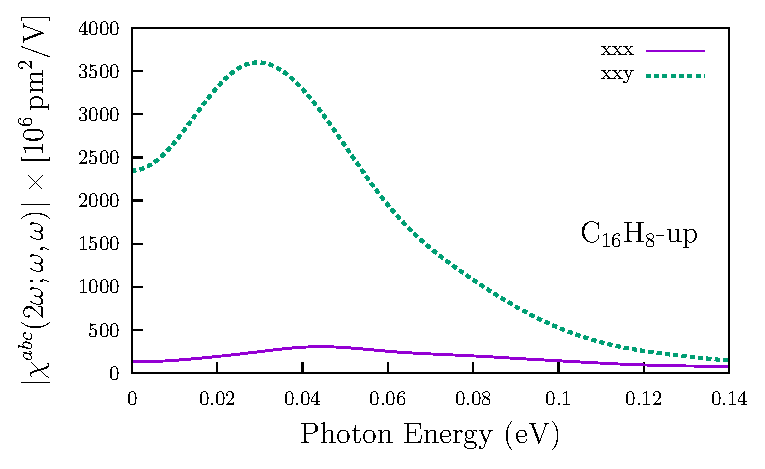
\includegraphics[width=\linewidth]{figures/up_shg_abs_x}}\\
% \subfloat{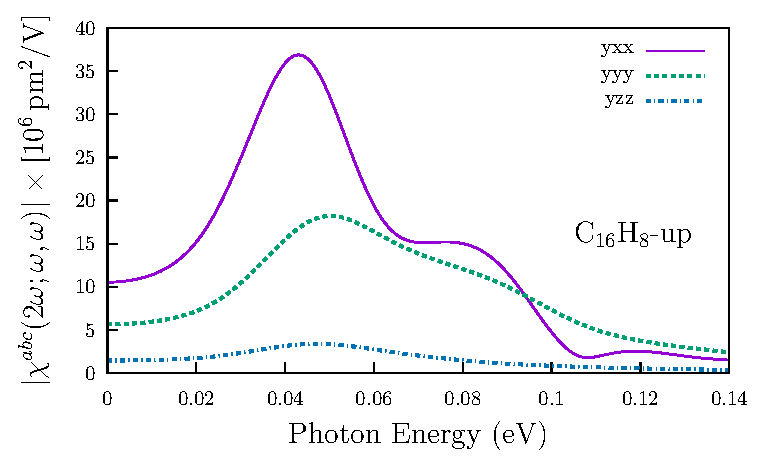
\includegraphics[width=\linewidth]{figures/up_shg_abs_y}}
% \caption{(Color online) Spectra of the absolute value of SHG for the
    % C$_{16}$H$_{8}$-up structure corresponding to the
    % sum of the absolute value for the non zero real and imaginary components
    % of $\chi^{abc}(2\omega;\omega,
    % \omega) $ tensor.\label{fig:up-shg-abs}}
% \end{figure}
% 
% \begin{table}[htb]%
% \sidecaption
% \begin{tabular}{lcccc}
% \hline
% Structure & \hspace{-5mm}Energy & \multicolumn{2}{c}{$\chi^{abc} $} &  Ref.\\
% \cline{3-4} & \hspace{-5mm}[eV] & $abc$ & value \\
% \hline
% C$_{16}$H$_{8}$-alt   & \hspace{-5mm}0.4   & xyy   & 0.32\scriptsize{$\times 10^{6}\,\mathrm{pm}^{2}/\mathrm{V}$}  & *     \\
% C$_{16}$H$_{8}$-up    & \hspace{-5mm}0.042 & yxx   & 37  \scriptsize{$\times 10^{6}\,\mathrm{pm}^{2}/\mathrm{V}$}  & *     \\
% Si(100)2$\times$1     & \hspace{-5mm}1.5   & xxx   & 1.5 \scriptsize{$\times 10^{6}\,\mathrm{pm}^{2}/\mathrm{V}$}  & \cite{andersonPRB15}  \\
% BNNT(6,0) pristine    & \hspace{-5mm}5.0   & zzz   & 35\,\scriptsize{pm/V}  & \cite{salazarPRB14} \\
% BNNT(6,0)+4(H$_{2}$)  & \hspace{-5mm}5.0   & zzz   & 33\,\scriptsize{pm/V}  & \cite{salazarPRB14} \\
% BNNT(6,0)+12(H$_{2}$) & \hspace{-5mm}4.8   & zzz   & 15\,\scriptsize{pm/V}  & \cite{salazarPRB14} \\
% \hline
% \end{tabular}
% \caption[]{%
% Comparison of the highest reported absolute values of SHG for 
  % different structures and components. ($^{*}$This work)}
% \label{tab:shgcomp}
% \end{table}


\section{Conclusions}\label{sec:conclusions}

We have performed \emph{ab initio} calculations for the optical spin injection (DSP), optical current injection (OCI), and second-harmonic generation (SHG) on the hydrogenated graphene C$_{16}$H$_{8}$-alt and C$_{16}$H$_{8}$-up structures, (Fig. \ref{fig:structures}) using the independent particle approximation (IPA) and the plane wabe basis. Our calculations abour DSP predicts that it is possible to inject spin-polarized electrons along the three cartesian directions, obtaining maxima DSP of the injected electrons of about 39\% and 57\% in the $y$ and $z$ directions  (Fig. \ref{fig:Da}) at the photon energies of around 0.719 and 0.08\,Ha  for the \emph{alt} and \emph{up} cases, respectively. Also there is a range of energy in which this DSP can be held,{\changed from 0.08 to 0.084\,eV and from 0.08 to 0.084\,eV for the \emph{alt} and \emph{up} cases, respectively}. This results predicts that particularly \emph{up} is usable for spintronics proposes because its energy is readily obtainable using terahertz radiation.

Our results about OCI with circularly polarized light (CPL) show that the \emph{alt}  and \emph{up} systems have a response near to 2.30\,mC$^{3}$/J$^{2}$s$^{2}$ and 18.0\,mC$^{3}$/J$^{2}$s$^{2}$ both in the $y$ direction (Figs. \ref{fig:alt-eta}-\ref{fig:up-eta}) for incident beams with energies of around 1.25 and 0.09\,eV. According to measurements done on bulk materials, it is actually possible to measure such amount of OCI. According to this result we can affir that it is possible to control the motion of electrons in both systems but specially in the \emph{up} one in the $y$ direction.

Finally we found that the \emph{alt} and \emph{up} structures present a absolute maximum of 0.32\,$\times10^{6} $\,pm$^{2}$/V and 37.0\,$\times10^{6} $\,pm$^{2}$/V at the photon energies of around 0.40\,eV and 0.042\,eV (Figs. \ref{fig:alt-shg-abs} and \ref{fig:up-shg-abs}). For \emph{alt} and \emph{up} we have that their maximua come from contributions of the 2$\omega$ resonances. From this we comclude that specially with the \emph{up} system is usable to SHG.


\section{Acknowledgment} % (fold)

This work has been supported by \emph{Consejo Nacional de Ciencia y
Tecnolog\'ia} (CONACyT), M\'exico, Grant No. 153930.


\bibliographystyle{pss}
\bibliography{graphane_structures}

\end{document}
